\documentclass[notitlepage]{article}
\usepackage[T1, T2A]{fontenc}
\usepackage[utf8]{inputenc}
\usepackage[russian]{babel}
%
%\usepackage{newtxmath}
%\usepackage {fouriernc} %bold
%\usepackage{kpfonts}
%%
%\usepackage{gentium}
%\usepackage[default]{droidserif}
%\usepackage{XCharter} %bold
%
\usepackage{tikz, enumerate, graphicx, amsmath, amssymb, physics, caption}
\usepackage[separate-uncertainty=true, 
exponent-product={}\cdot, output-decimal-marker={,}]{siunitx}
\usetikzlibrary{calc,intersections, decorations.pathreplacing}
\newcommand{\intl}{\int\limits}
\newcommand{\intlinf}{\int\limits_{-\infty}^{+\infty}}
\newcommand\inner[2]{\left\langle #1, #2 \right\rangle}
\newcommand{\yav}[2]{\num{#1}\,\text{#2}}
\let\epsilon\varepsilon
\newcommand{\fpageplot}[4][90]
{\begin{figure}
  \caption{#4}
  \includegraphics[angle=#1, height=\textheight, width=\textwidth, keepaspectratio]
  {#2}
  \label{#3}
\end{figure}
}
\usepackage[a4paper, left=2cm, right=2cm, top=3cm, bottom=3cm]{geometry}
\title{Второе задание по методам оптимизации}
\author{Иван Ермаков}
\date{}
\begin{document}
\maketitle
\section*{3}
Логистическая регрессия
\begin{equation}
  \min_{x \in \mathbb{R}^n} \left\{f(x) = \frac 1m\inner{\ln\left[1 + \exp\left(-b \odot \left(A x\right)\right)\right]}{1_m}
  + \frac{\lambda}2 \norm{x}^2\right\}
\end{equation}
Здесь $b$ --- вектор из $b_i$, $A^T$ -- матрица $m \times n$, в которой строки являются векторами $a_i$.

\begin{equation}
  \begin{aligned}
    \operatorname{D} f(x) &= \lambda x - \frac {A^T} m\left(b\odot\frac{\exp\left(-b \odot \left(A x\right)\right)}
  {1 + \exp\left(-b \odot \left(A x\right)\right)}\right) = 
  \lambda x - \frac {A^T} m\left(b\odot u\left[-b\odot \left(A x\right)\right]\right)\\
  u(y) &= \frac{e^y}{1 + e^y} = \frac1{1 + e^{-y}}
  \end{aligned}
\end{equation}
Здесь использовано много свойств произведения Адамара.

\begin{equation}
    \dv{u}{y} = \frac{e^y(1 + e^y) - e^{2y}}{(1 + e^y)^2} = \frac{e^y}{(1 + e^y)^2}\\
    \end{equation}
\begin{equation}
  \operatorname{D}^2 f[\dd x] = \lambda \dd x + \frac {A^T}m \left(b\odot \frac{e^y}{(1 + e^y)^2} \odot b \odot \left(A \dd x \right)\right)
    \end{equation}
\begin{equation}
  \operatorname{D}^2 f = 
  \lambda + \frac {A^T}m \left\{\left[\left(b \odot b \odot \frac{e^y}{(1 + e^y)^2}[-b \odot (Ax)]\right) 1_n^T\right] \odot A\right\}
\end{equation}
Потратив еще \textit{немного} времени, можно понять, что это выражение можно переписать как
\begin{equation}
  \operatorname{D}^2 f = \lambda + \frac 1m \cdot A^T \operatorname{diag}\left\{b\odot b \odot v(-b \odot \left(A x\right))\right\} A
\end{equation}
где
\begin{equation}
  v(y) = \frac{e^y}{(1 + e^y)^2}
\end{equation}
\section{Эксперимент: траектория градиентного спуска}
Построение графиков выполнено при помощи скрипта ``gradplots/trajectory.py''. 
\begin{figure}[ht]
\begin{minipage}[t]{.5\textwidth}
  \centering
  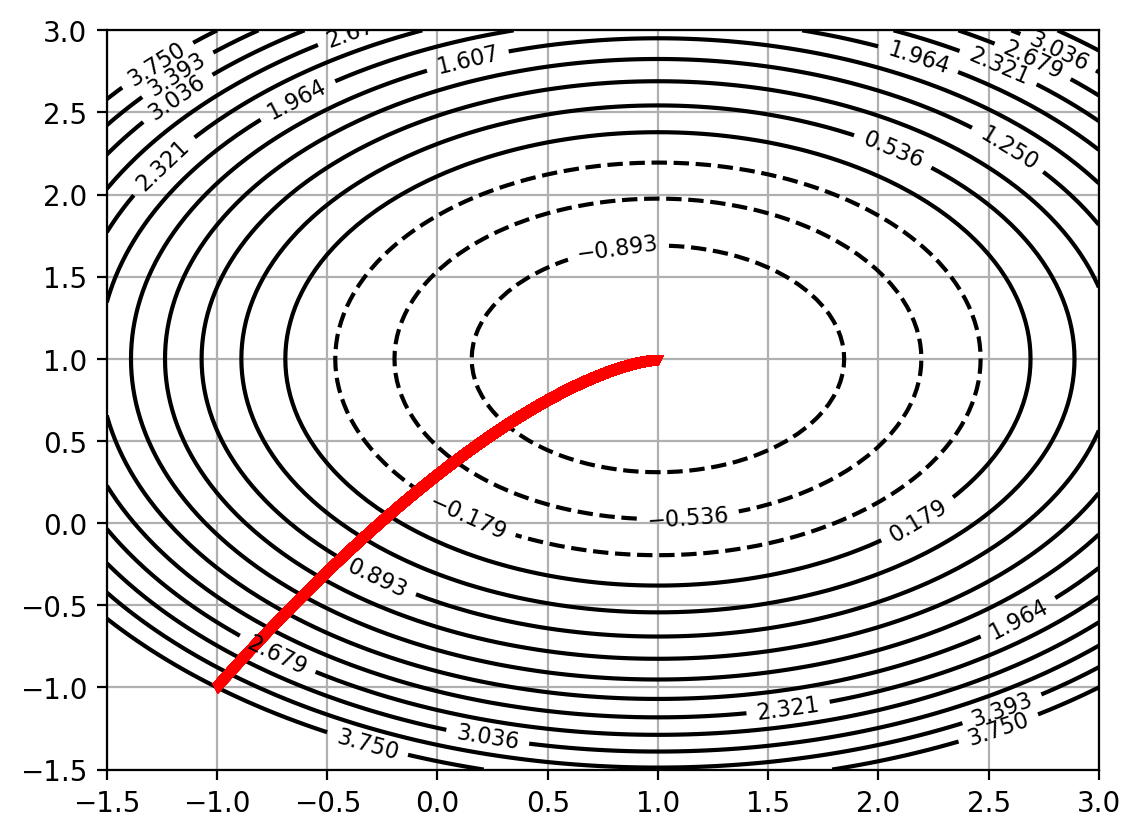
\includegraphics[width=\textwidth, keepaspectratio]{plots/trajectory_0_0.png}
  \captionof{figure}{Постоянный шаг, хорошо обусловленная матрица.}
\end{minipage}
\begin{minipage}[t]{.5\textwidth}
  \centering
  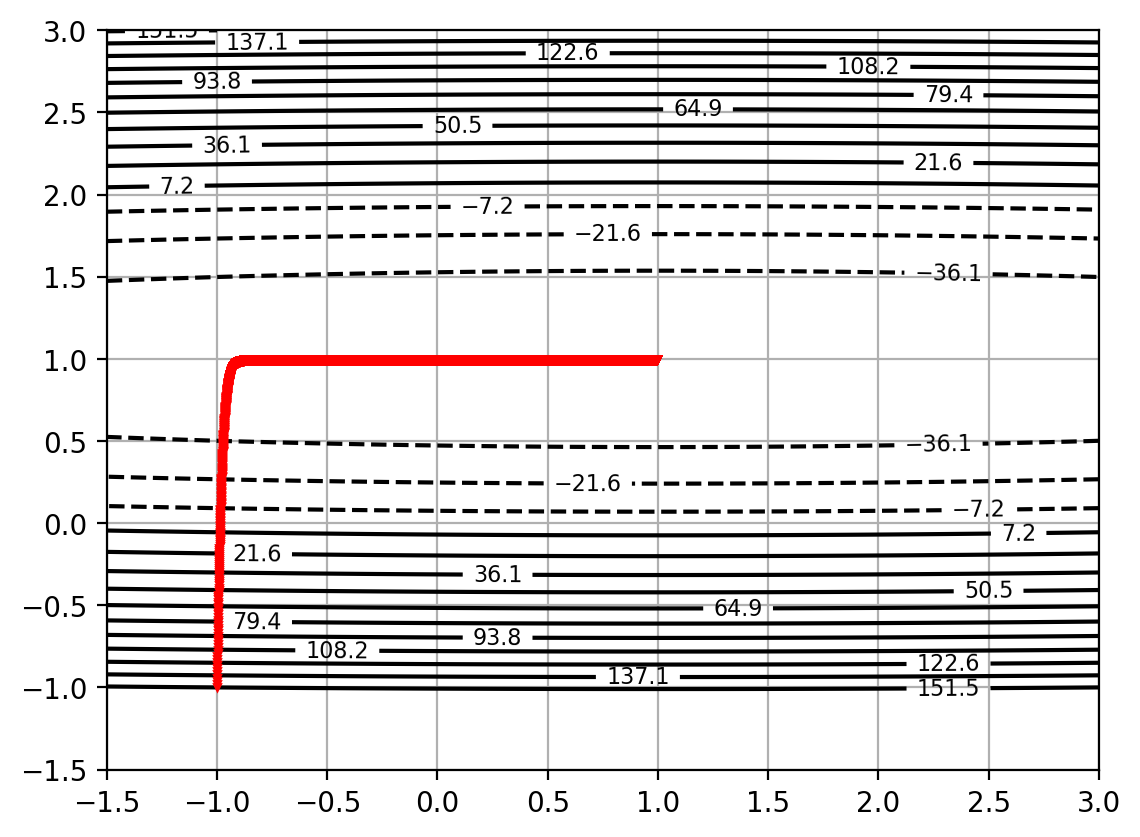
\includegraphics[width=\textwidth, keepaspectratio]{plots/trajectory_1_0.png}
  \captionof{figure}{Постоянный шаг, плохо обусловленная матрица.}
\end{minipage}
\end{figure}
Для хорошо обусловленной матрицы поиск останавливается за 109000 шагов, а для плохо обусловленной за 69000.
Скорее всего так происходит из-за того, что в хорошо обсусловленной матрице метод постоянно проскакивает оптимальную точку
из-за высокой требуемой точности.

\begin{figure}[ht]
\begin{minipage}[t]{.5\textwidth}
  \centering
  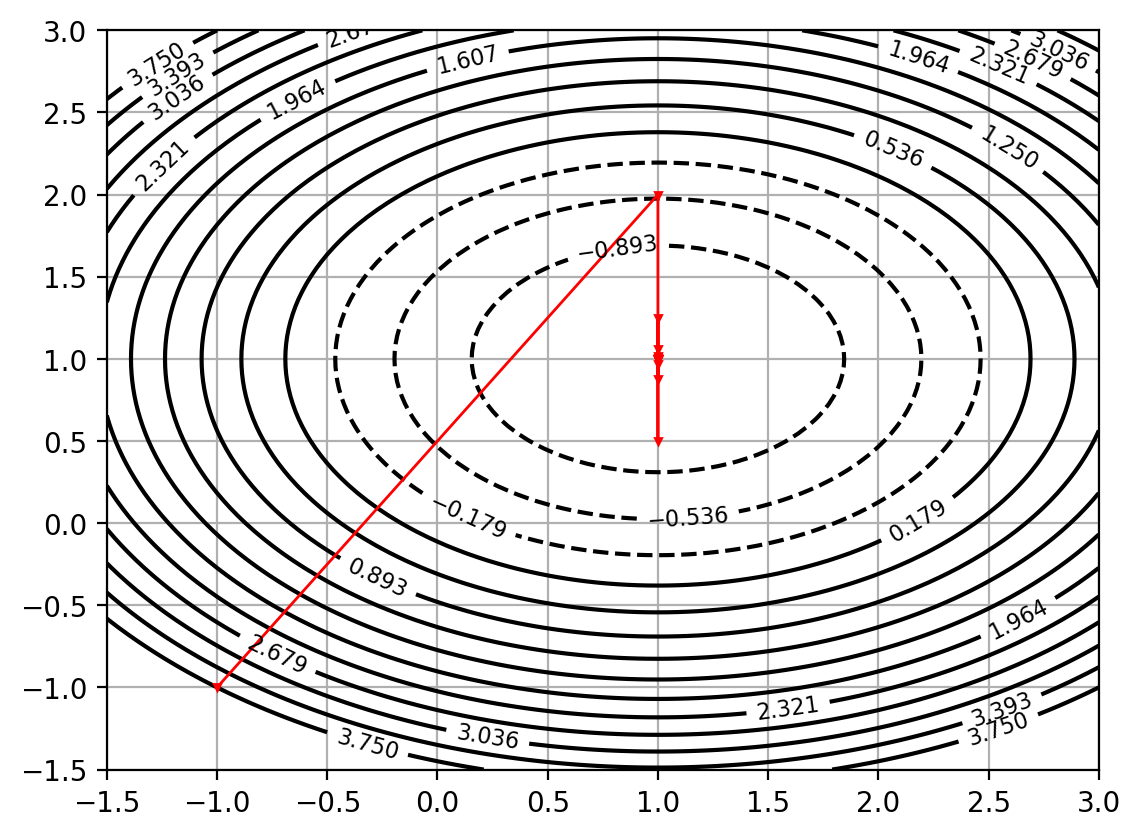
\includegraphics[width=\textwidth, keepaspectratio]{plots/trajectory_0_1.png}
  \captionof{figure}{Условие Армихо, хорошо обусловленная матрица.}
\end{minipage}
\begin{minipage}[t]{.5\textwidth}
  \centering
  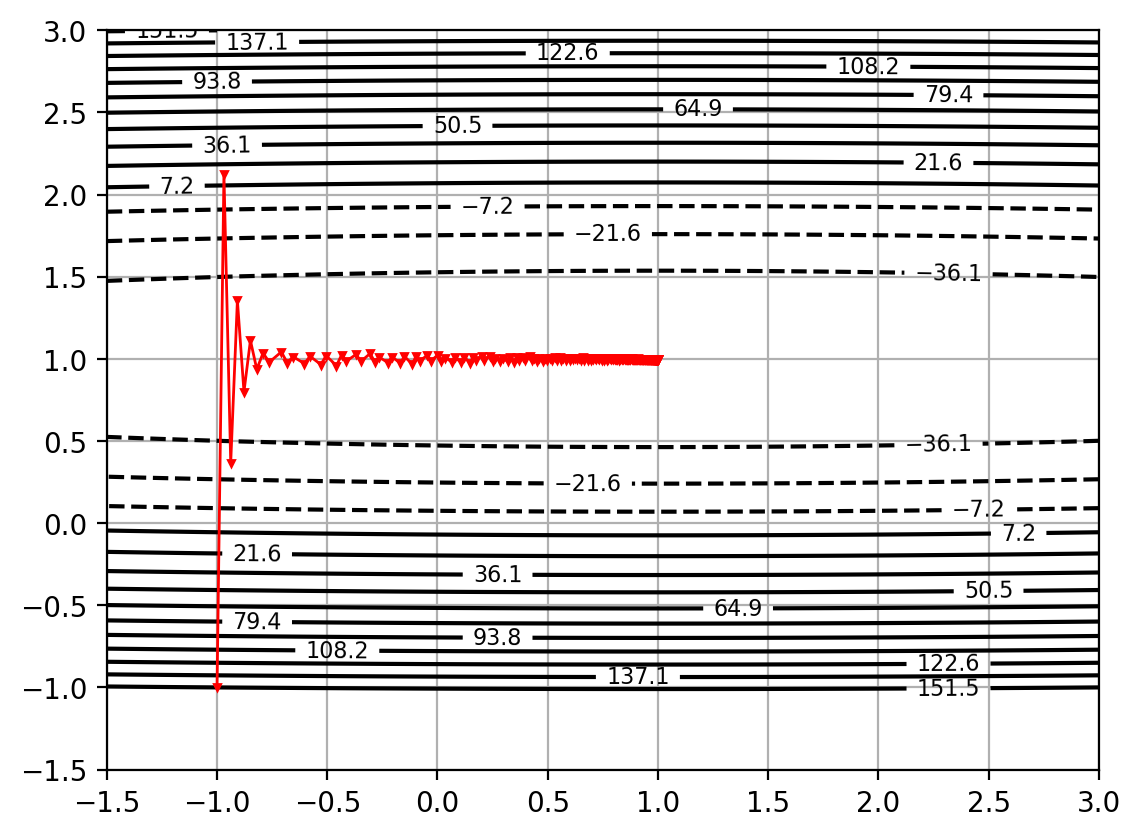
\includegraphics[width=\textwidth, keepaspectratio]{plots/trajectory_1_1.png}
  \captionof{figure}{Условие Армихо, плохо обусловленная матрица.}
\end{minipage}
\end{figure}
Теперь все встало на свои места: для хорошо обусловленной матрицы метод сходится всего за 18 шагов. Для плохо обусловленной
требуется 327 шагов. Видно, что в первом случае довольно быстро тракетория становится прямой, а во втором случае она все время
колеблется вокруг оптимального пути и совершает больше шагов, чем нужно.

\begin{figure}[ht]
\begin{minipage}[t]{.5\textwidth}
  \centering
  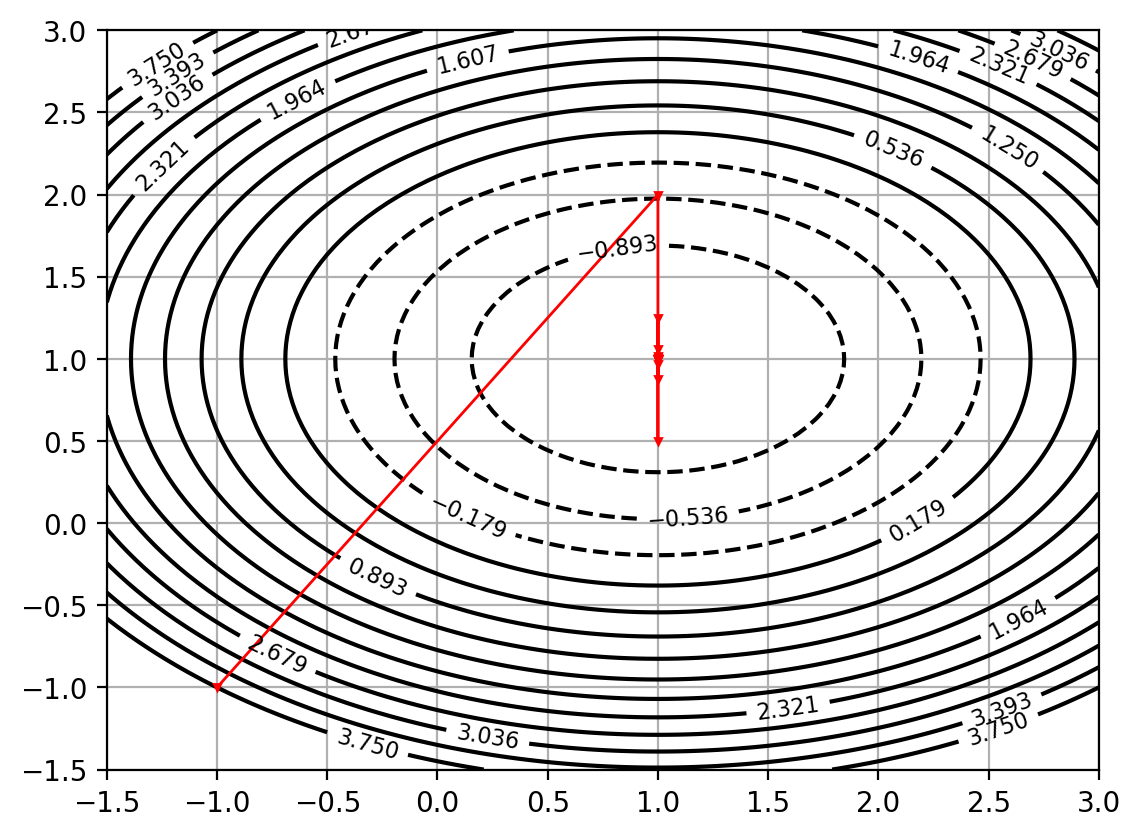
\includegraphics[width=\textwidth, keepaspectratio]{plots/trajectory_0_2.png}
  \captionof{figure}{Условие Вольфа, хорошо обусловленная матрица.}
\end{minipage}
\begin{minipage}[t]{.5\textwidth}
  \centering
  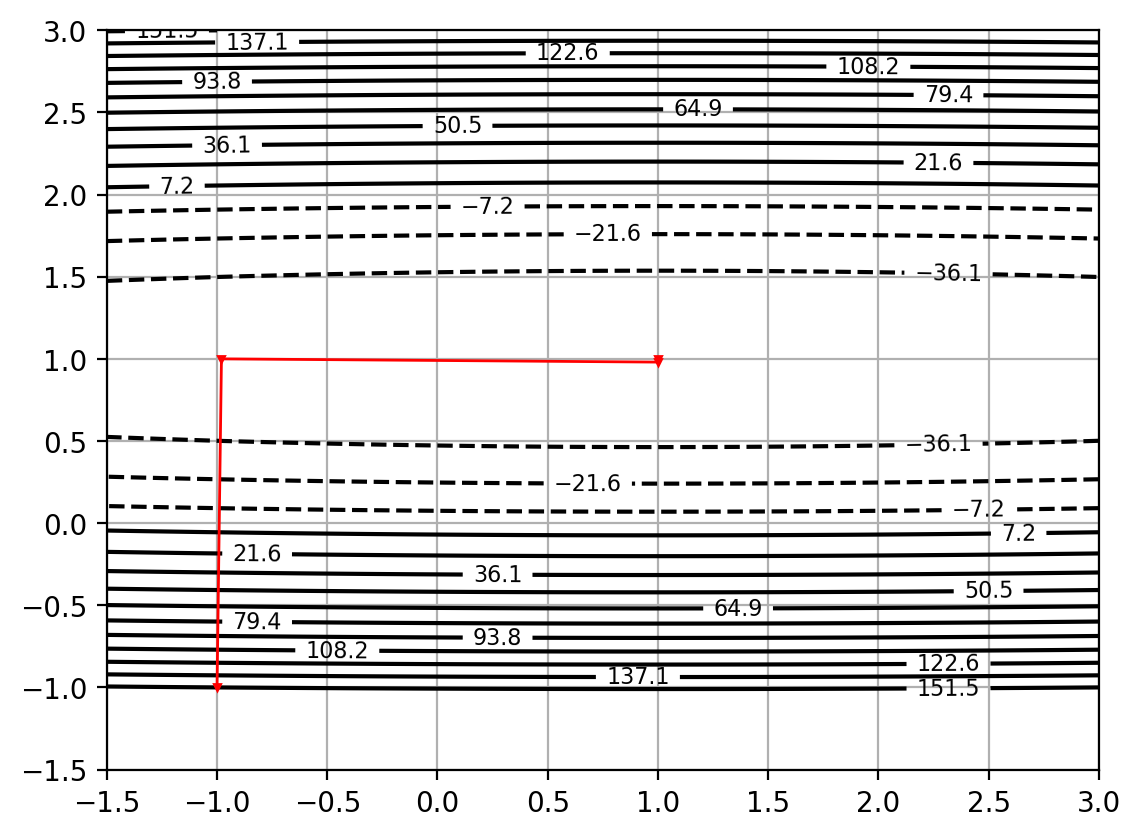
\includegraphics[width=\textwidth, keepaspectratio]{plots/trajectory_1_2.png}
  \captionof{figure}{Условие Вольфа, плохо обусловленная матрица.}
\end{minipage}
\end{figure}
Для условия Вольфа ситуация аналогичная первому случаю: для хорошо обусловленной матрицы метод работает ``слишком хорошо'' и
проскакивает точку экстремума. Метод сходится за 18 шагов. Для плохо обусловленной матрицы требуется всего 4 шага.
Понятно, что в общем случае для хорошо обусловленой матрицы метод Вольфа тоже работает хорошо, и некоторое $O(1)$ количество
операций в конце, связанное с проскакиванием, роли не играет.

При этом, конечно, чем ближе прямая градиента к оптимальной точке, тем быстрее будут работать все методы, потому что траектория будет
ближе к прямой.
			
			
\end{document}
